Introducción al capítulo

%--------------------------------------------------
\section{Objetivos}

% - - - - - - - - - - - - - - - - - - - - - - - - -
\subsection{Objetivo general}

% - - - - - - - - - - - - - - - - - - - - - - - - -
\subsection{Objetivos específicos}

%--------------------------------------------------
\section{Modelo de despliegue}


% - - - - - - - - - - - - - - - - - - - - - - - - -
\subsection{Requerimientos no funcionales}


% - - - - - - - - - - - - - - - - - - - - - - - - -
\subsection{Modelo de despliegue del sistema}

Diagrama de despliegue presentando los sistemas (comunicaciones, sistemas externos y software de base) con los que interactúa el sistema y su explicación. vea los siguientes cuatro ejemplos.

	\begin{figure}[htbp!]
		\centering
			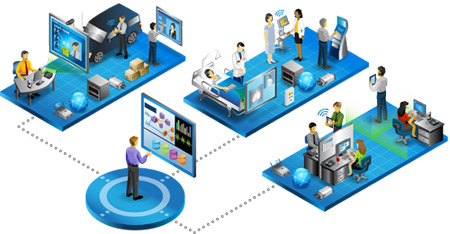
\includegraphics[width=0.8\textwidth]{images/arquitectura1}
		\caption{Diagrama de arquitectura.}
	\end{figure}

	\begin{figure}[htbp!]
		\centering
			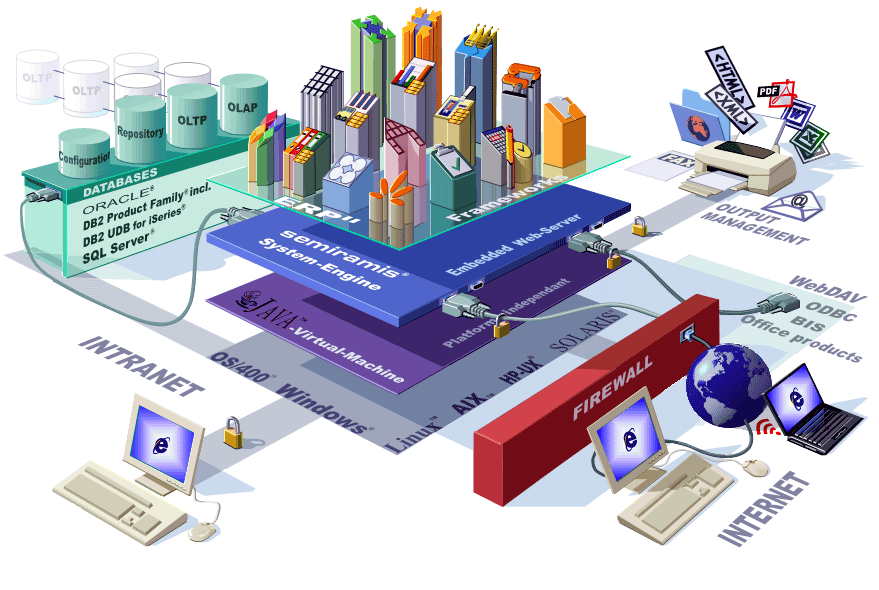
\includegraphics[width=0.8\textwidth]{images/arquitectura2}
		\caption{Diagrama de arquitectura.}
	\end{figure}

	\begin{figure}[htbp!]
		\centering
			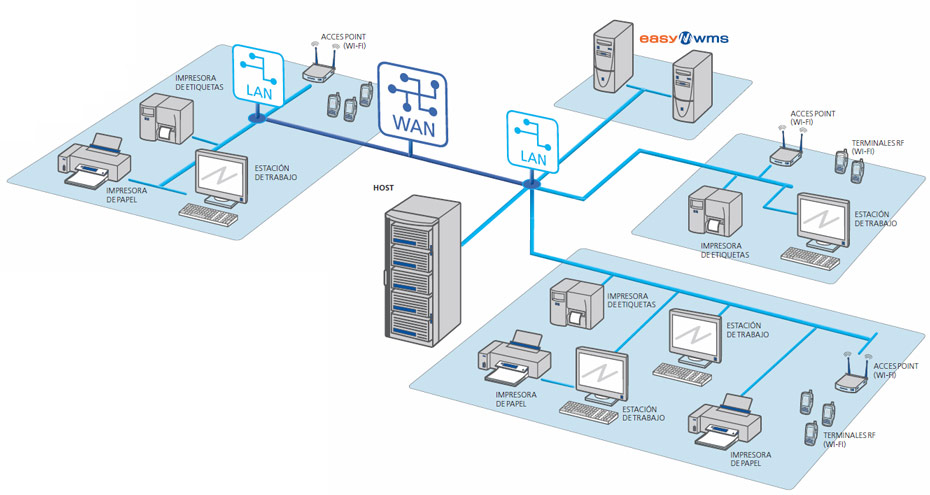
\includegraphics[width=0.8\textwidth]{images/arquitectura3}
		\caption{Diagrama de arquitectura.}
	\end{figure}

	\begin{figure}[htbp!]
		\centering
			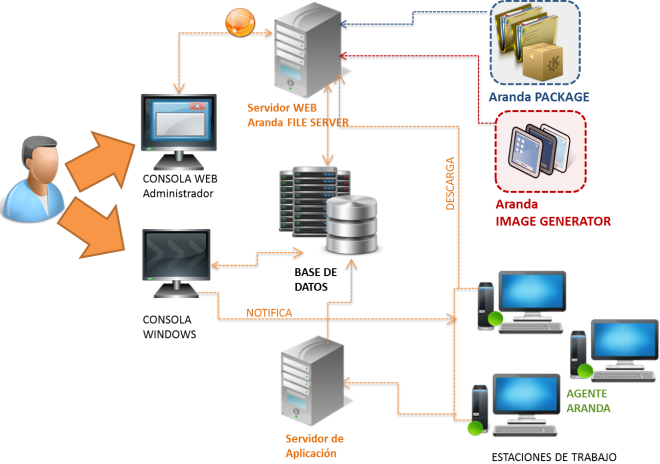
\includegraphics[width=0.8\textwidth]{images/arquitectura4}
		\caption{Diagrama de arquitectura.}
	\end{figure}


% - - - - - - - - - - - - - - - - - - - - - - - - -
\subsection{Especificación de Plataforma}

Especificar, hardware, software y servicios requeridos para el sistema.

